\chapter{Funktionsgliederung/-Struktur}
	% Um das Gerät strukturiert konstruieren zu können, werden die einzelnen Funktionen, welche der Arm erfüllen soll, gegliedert.
	Zur Zwecke der Reduktion des Komplexitätsgrades des Gesamtsystems wird sich für das Erstellen eines Funktionsbaumes entschieden.
	Hier werden die in \cref{chap:Aufgabenstellung} formulierten Anforderungen in grober Form vorstrukturiert um sich einen Überblick über die Anzahl und Gestalt funktionaler Teilprobleme, sowie möglicher Lösungsansätze zu verschaffen.
	Hieraus können in einer frühen Konzeptionsphase bereits unpraktikable Lösungsansätze verworfen und in der textlichen Ausformulierung gegebenenfalls verborgen gebliebene Teilprobleme identifiziert werden.
	Im direkten Anschluss können Kernfunktionen und/oder Lösungsansätze im Rahmen morphologischer Kästen weiter diskutiert werden.	Wie feingliedrig dies geschehen soll, liegt im Ermessen der Konstrukteure.

\section{Funktionsbaum}
	Zunächst werden die allgemeinen Funktionen in Kategorien unterteilt, um eine Übersicht zu erschaffen. Diese sind in einem Funktionsbaum (s. \cref{fig:funktionsbaum}) zu sehen.

	\begin{figure}[h]
		\centering
		\includesvg[height=.75\textheight]{Abb/chart}
		% \includesvg[width=\textwidth]{Abb/chart}
		\caption[Funktionsbaum]{Funktionsbaum.}
		\label{fig:funktionsbaum}
	\end{figure}


\section{Morphologische Kästen}
	% Im nächsten Schritt sind die erforderlichen Funktionen und mögliche Lösungen in morphologische Kästen (s. \crefrange{fig:morphologische-kasten-teilprobleme}{fig:morphologische-kasten-feedback-system}) aufgestellt. Die von uns gewählten Lösungen sind in grün markiert.\\
	% Die Begründungen zu den Lösungsauswahlen werden in \cref{Begründung Lösungsauswahl} näher erläutert.
	Zunächst wurden aus dem Funktionsbaum kritische Probleme abgeleitet und als Teilprobleme in morphologischen Kästen (s. \crefrange{fig:morphologische-kasten-teilprobleme}{fig:morphologische-kasten-feedback-system}) dargestellt. Da einige Bauteile viele Teilprobleme aufwiesen, wurden diese in eigenen morphologischen Kästen behandelt. Im Anschluss wurde zu den entsprechenden Problemen Lösungen gesucht und diese dargestellt. Die Lösungen beruhen auf dem Wissen und der Erfahrung des Konstruktionsteams. Die Lösungen wurden danach im Hinblick auf verschiedene Kriterien überprüft und die passendste Lösung gewählt. Entscheidende Kriterien dabei waren die Komplexität, die Herstellbarkeit sowie die Kosten.

	\begin{table}[h]
		\centering
		\caption[Morphologischer Kasten der Teilprobleme]{Morphologischer Kasten der Teilprobleme.}
		\centering
		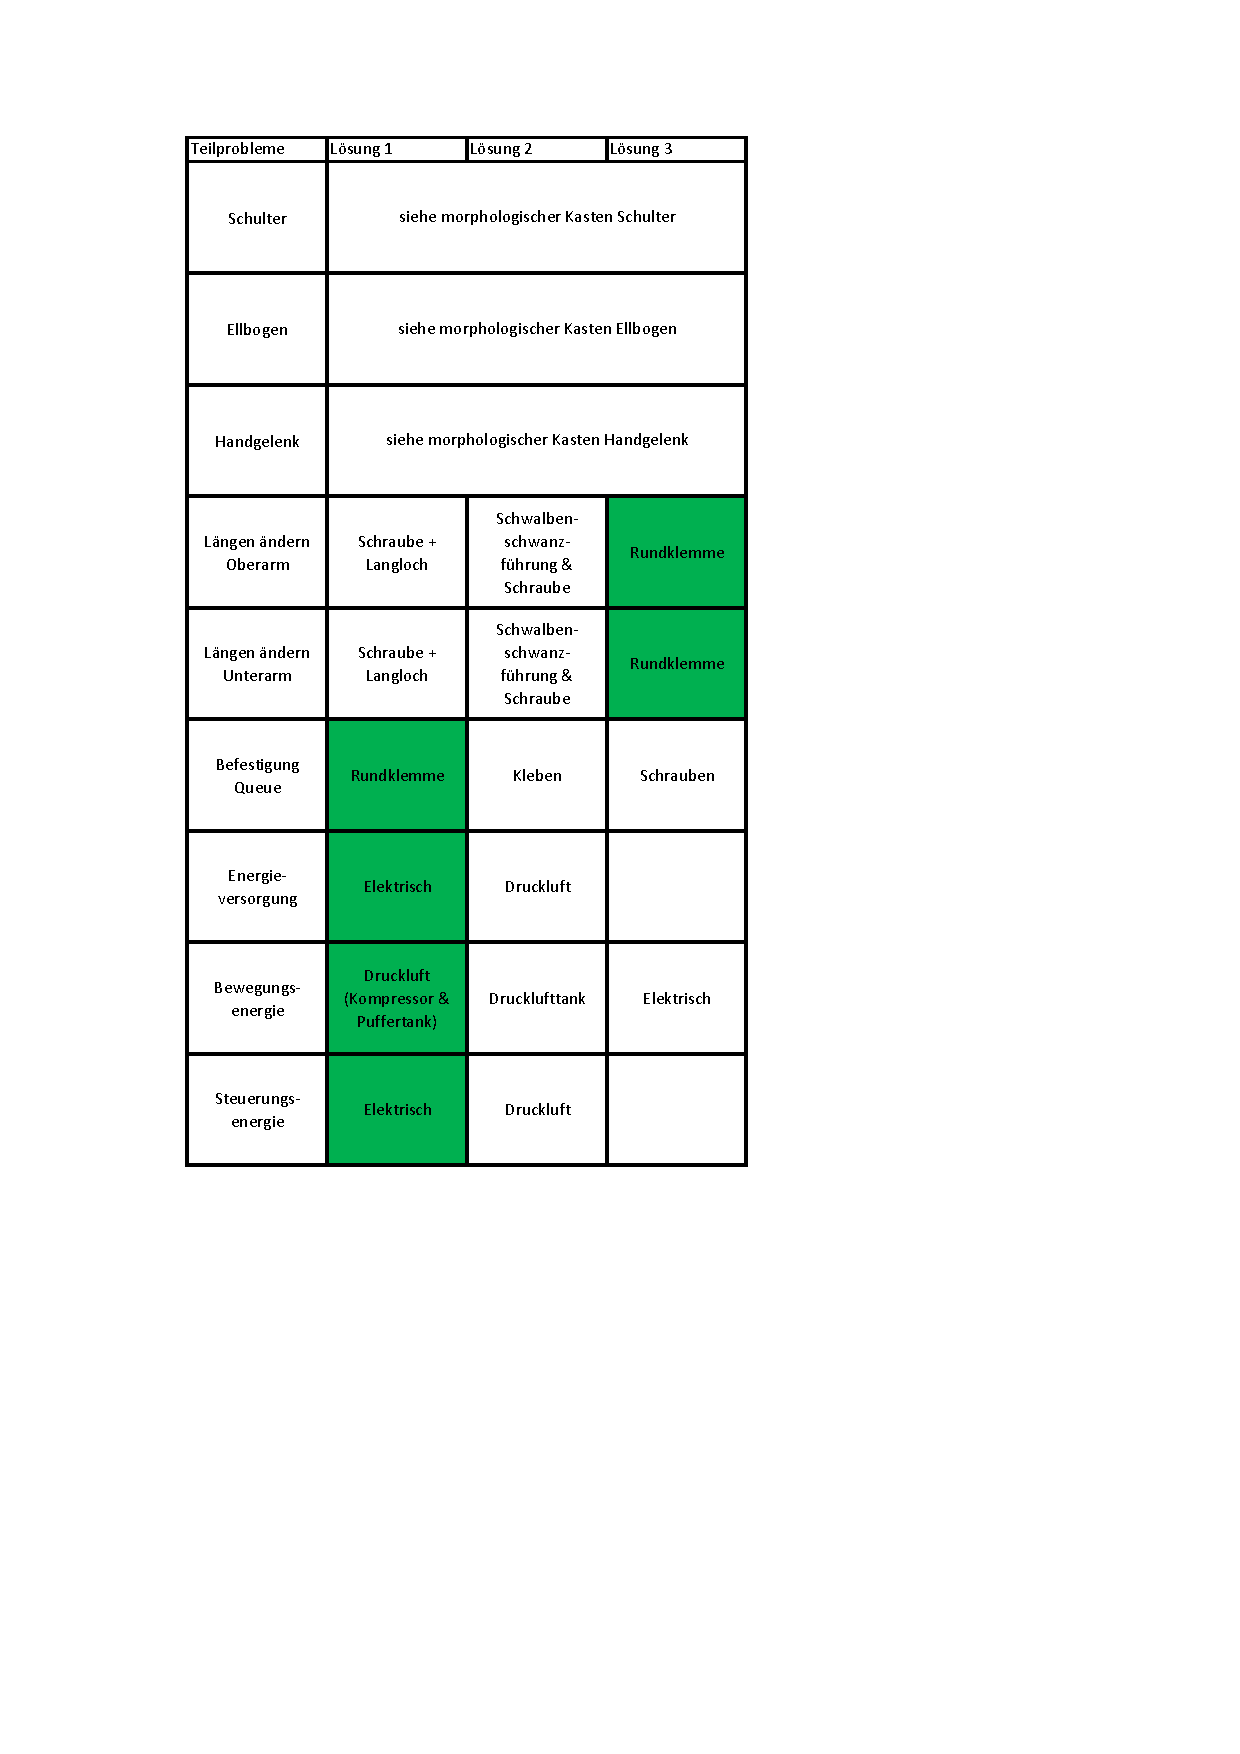
\includegraphics[width=\textwidth]{Abb/Morphologischer_Kasten_Teilprobleme}
		\label{fig:morphologische-kasten-teilprobleme}
	\end{table}

	\begin{table}[h]
		\caption[Morphologischer Kasten der Schulter]{Morphologischer Kasten der Schulter.}
		\centering
		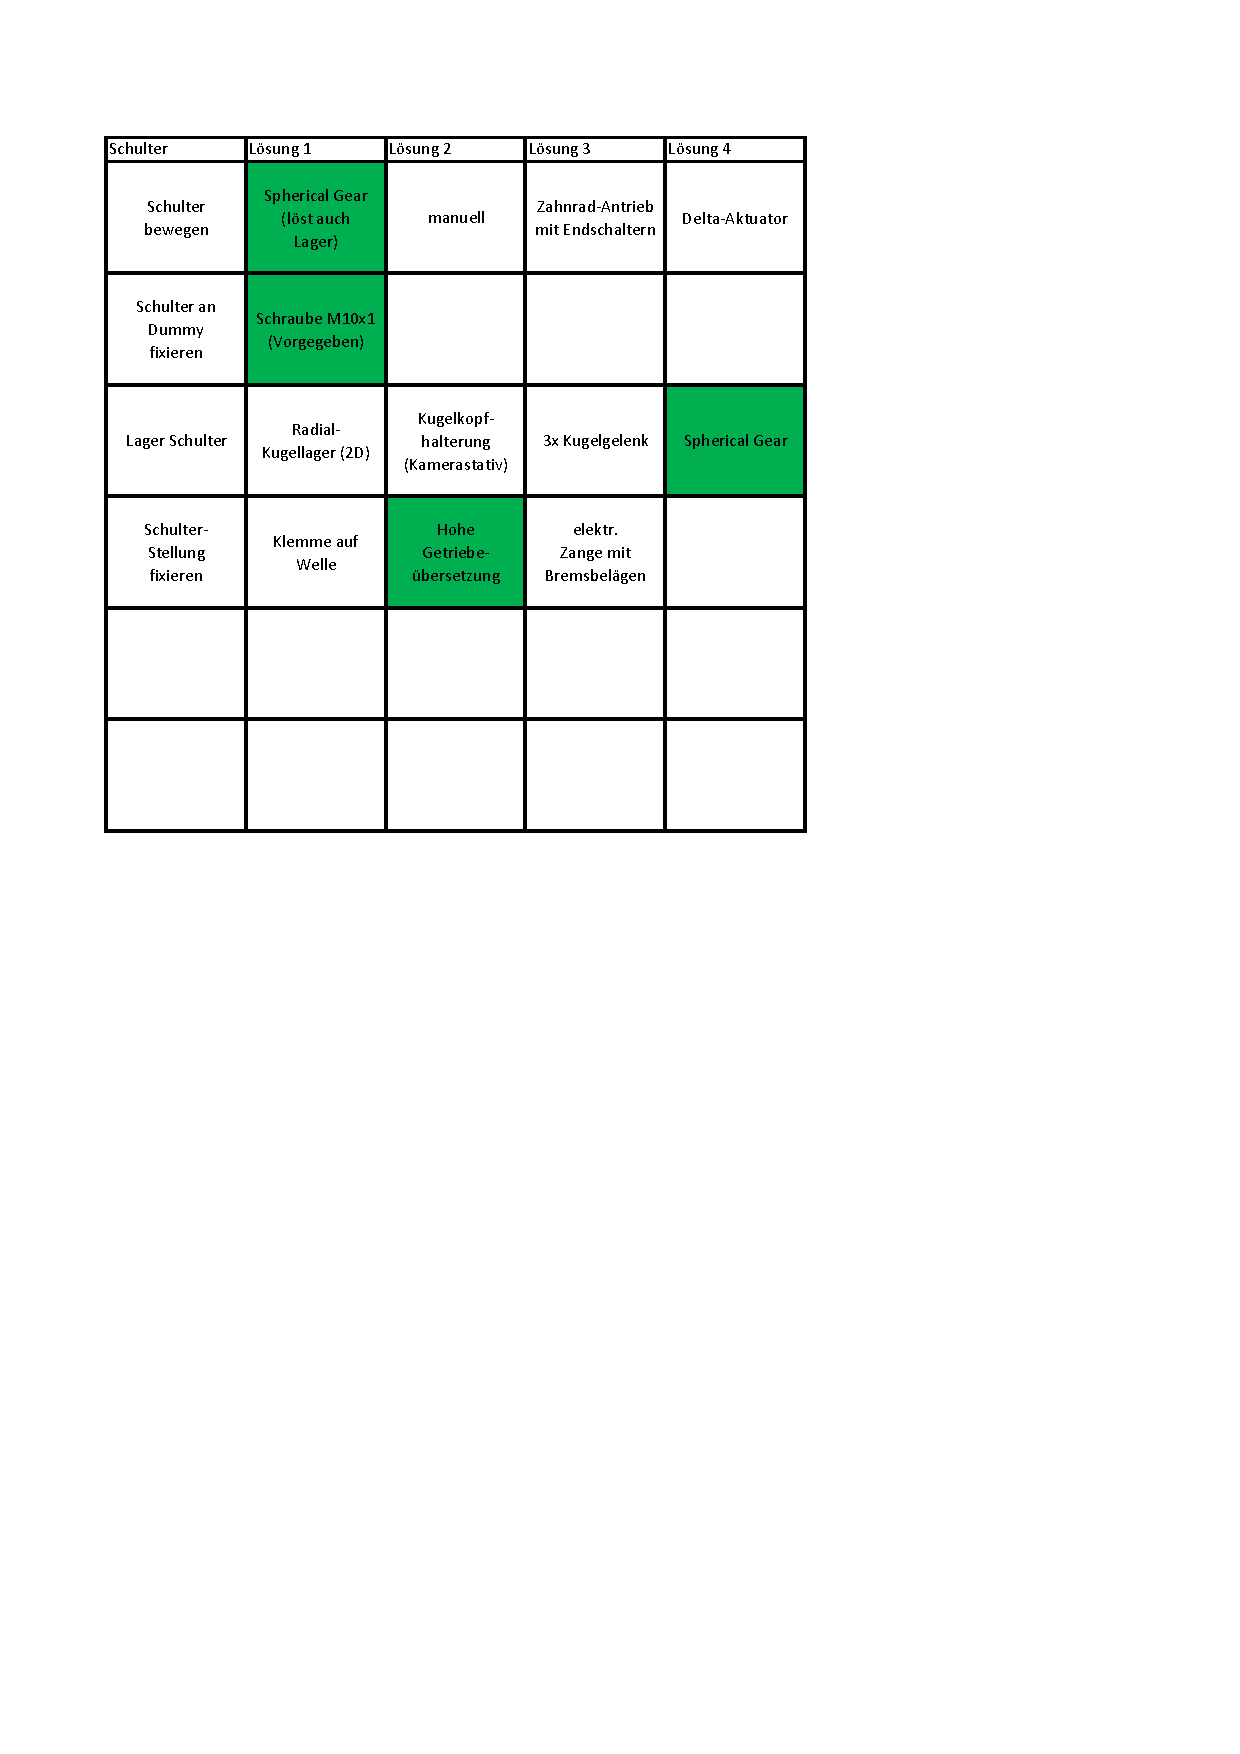
\includegraphics[width=\textwidth]{Abb/Morphologischer_Kasten_Schulter}
		\label{fig:morphologische-kasten-schulter}
	\end{table}

	\begin{table}[h]
		\caption[Morphologischer Kasten des Ellbogens]{Morphologischer Kasten des Ellbogens.}
		\centering
		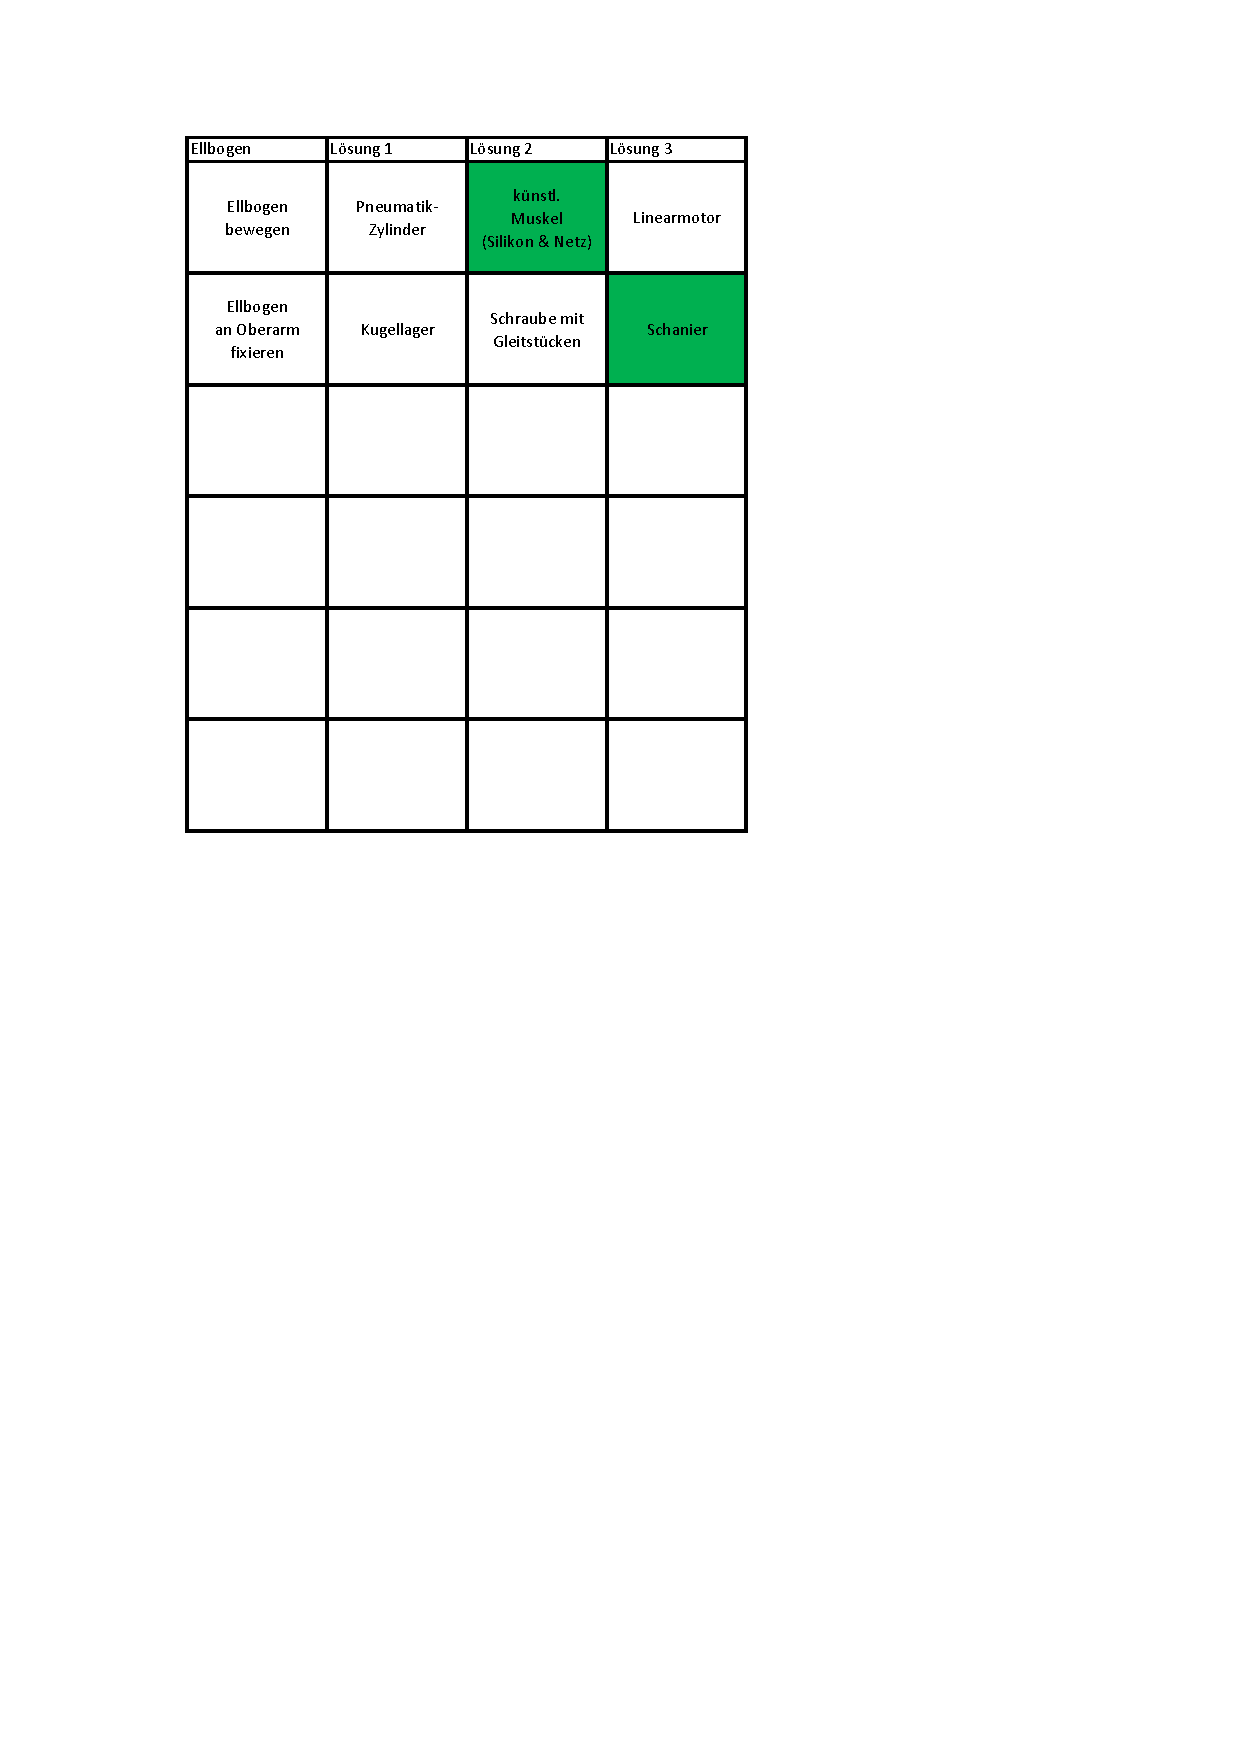
\includegraphics[width=\textwidth]{Abb/Morphologischer_Kasten_Ellbogen}
		\label{fig:morphologische-kasten-ellbogen}
	\end{table}

	\begin{table}[h]
		\caption[Morphologischer Kasten des Handgelenks]{Morphologischer Kasten des Handgelenks.}
		\centering
		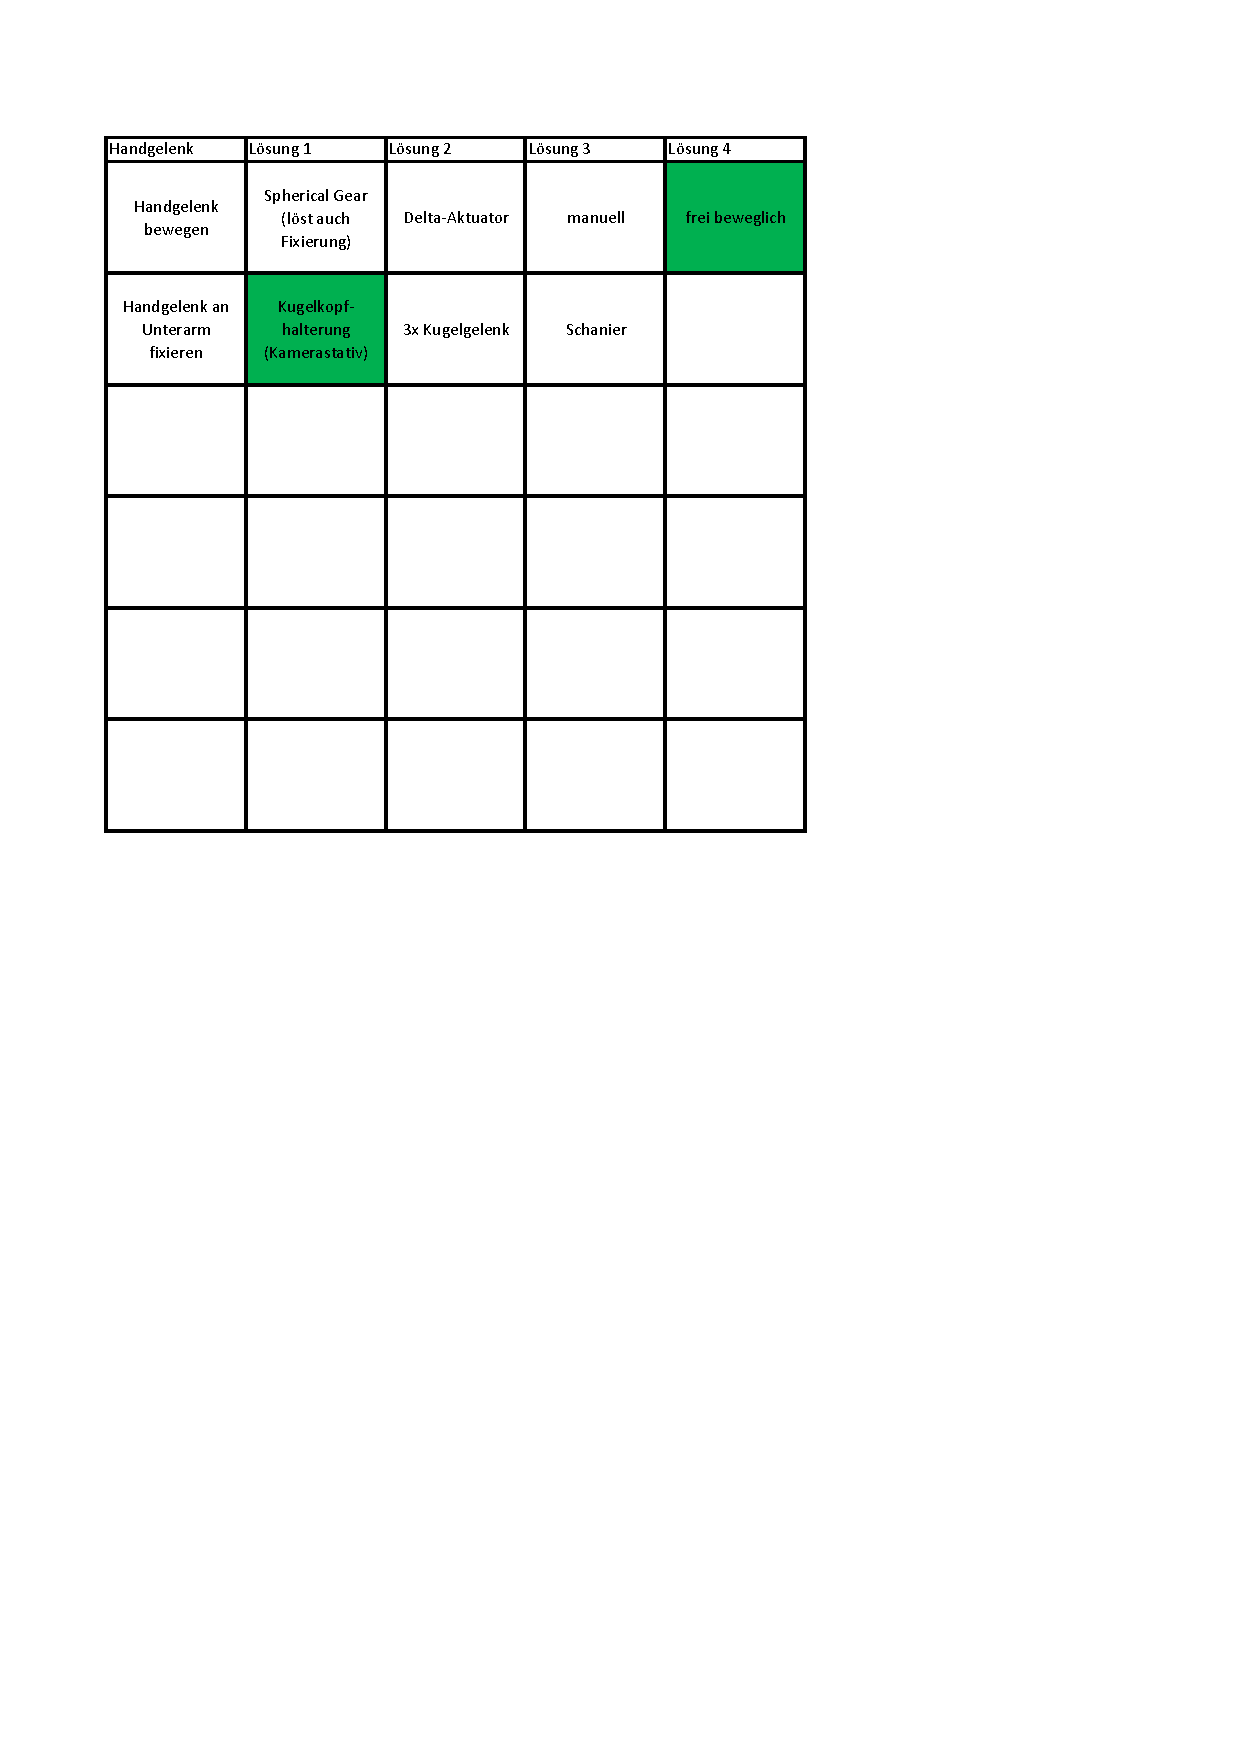
\includegraphics[width=\textwidth]{Abb/Morphologischer_Kasten_Handgelenk}
		\label{fig:morphologische-kasten-handgelenk}
	\end{table}

	\begin{table}[h]
		\caption[Morphologischer Kasten des Feedback-Systems]{Morphologischer Kasten des Feedback-Systems.}
		\centering
		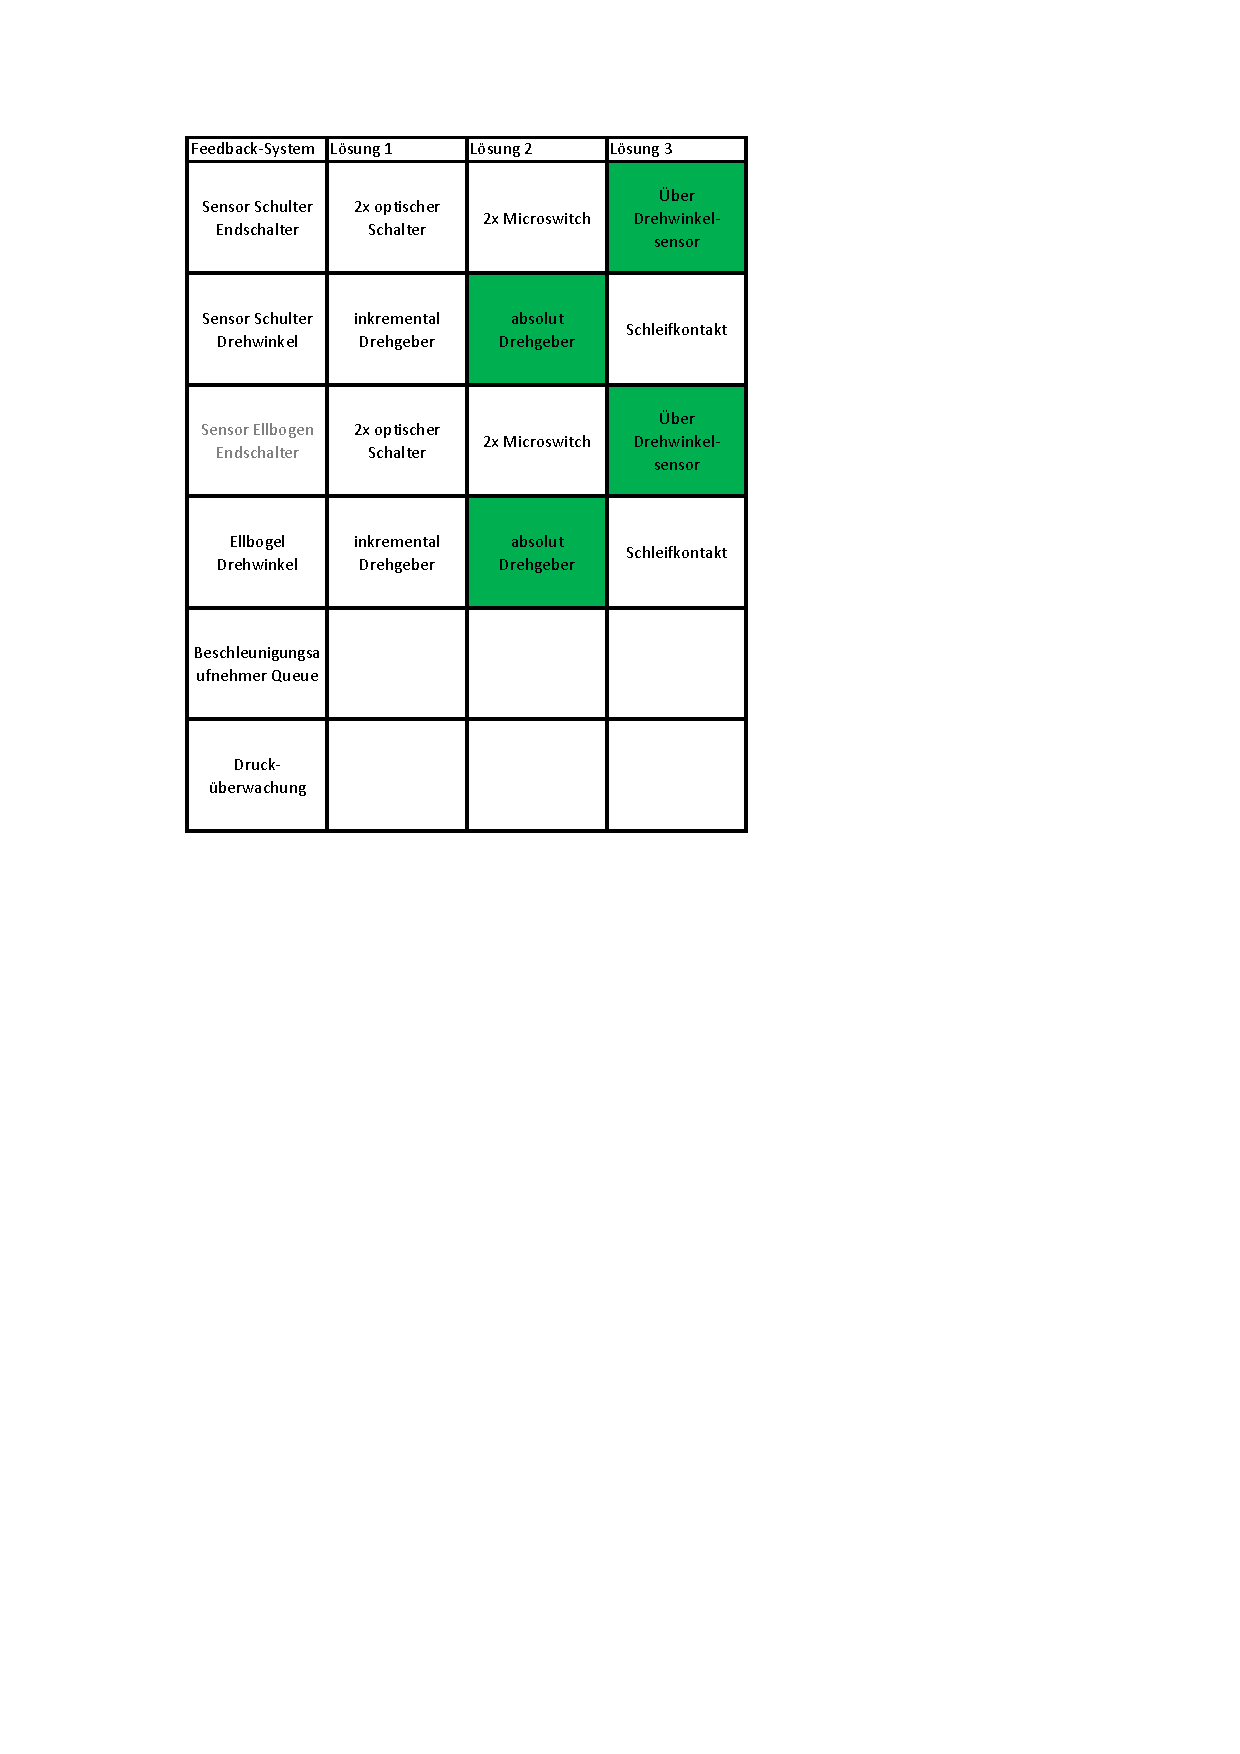
\includegraphics[width=\textwidth]{Abb/Morphologischer_Kasten_Feedback-System}
		\label{fig:morphologische-kasten-feedback-system}
	\end{table}

\section{Prinzipskizze}
	Da die Funktionen nun definiert sind, kann das Prinzip des Gerätes schematisch in einer Prinzipskizze aufgezeigt werden.\\
	\cref{fig:prinzipskizze-gesamtansicht} zeigt die Hauptbauteile, \cref{fig:prinzipskizze-ellbogen} den Anschluss zwischen Ober- und Unterarm und \cref{fig:prinzipskizze-handgelenk-und-hand} die Hand und ihre Verbindung zum Unterarm.

	\begin{figure}[h]
		\centering
		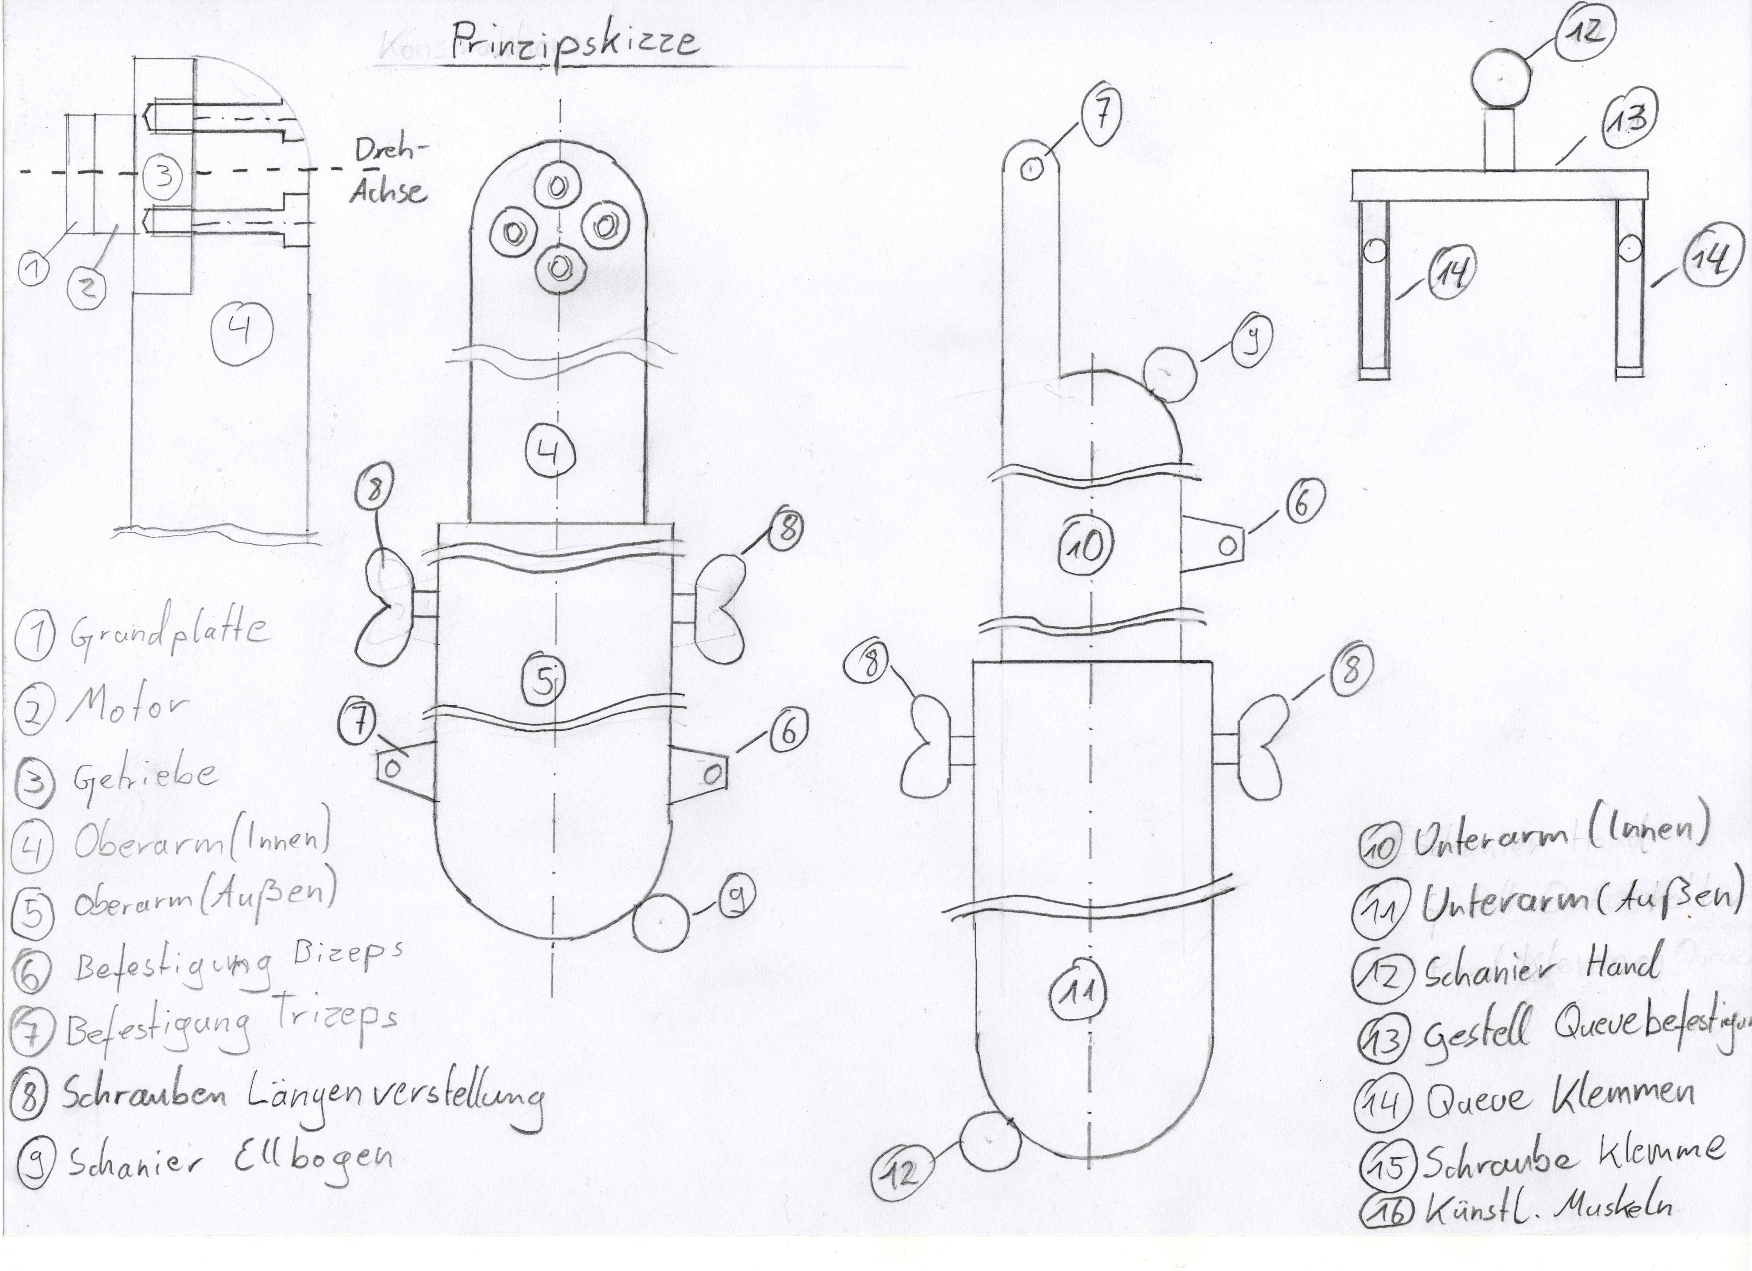
\includegraphics[width=\textwidth]{Abb/Prinzipskizze_Gesamtansicht}
		\caption[Prinzipskizze -- Gesamtansicht]{Prinzipskizze -- Gesamtansicht.}
		\label{fig:prinzipskizze-gesamtansicht}
	\end{figure}

	\begin{figure}[h]
		\centering
		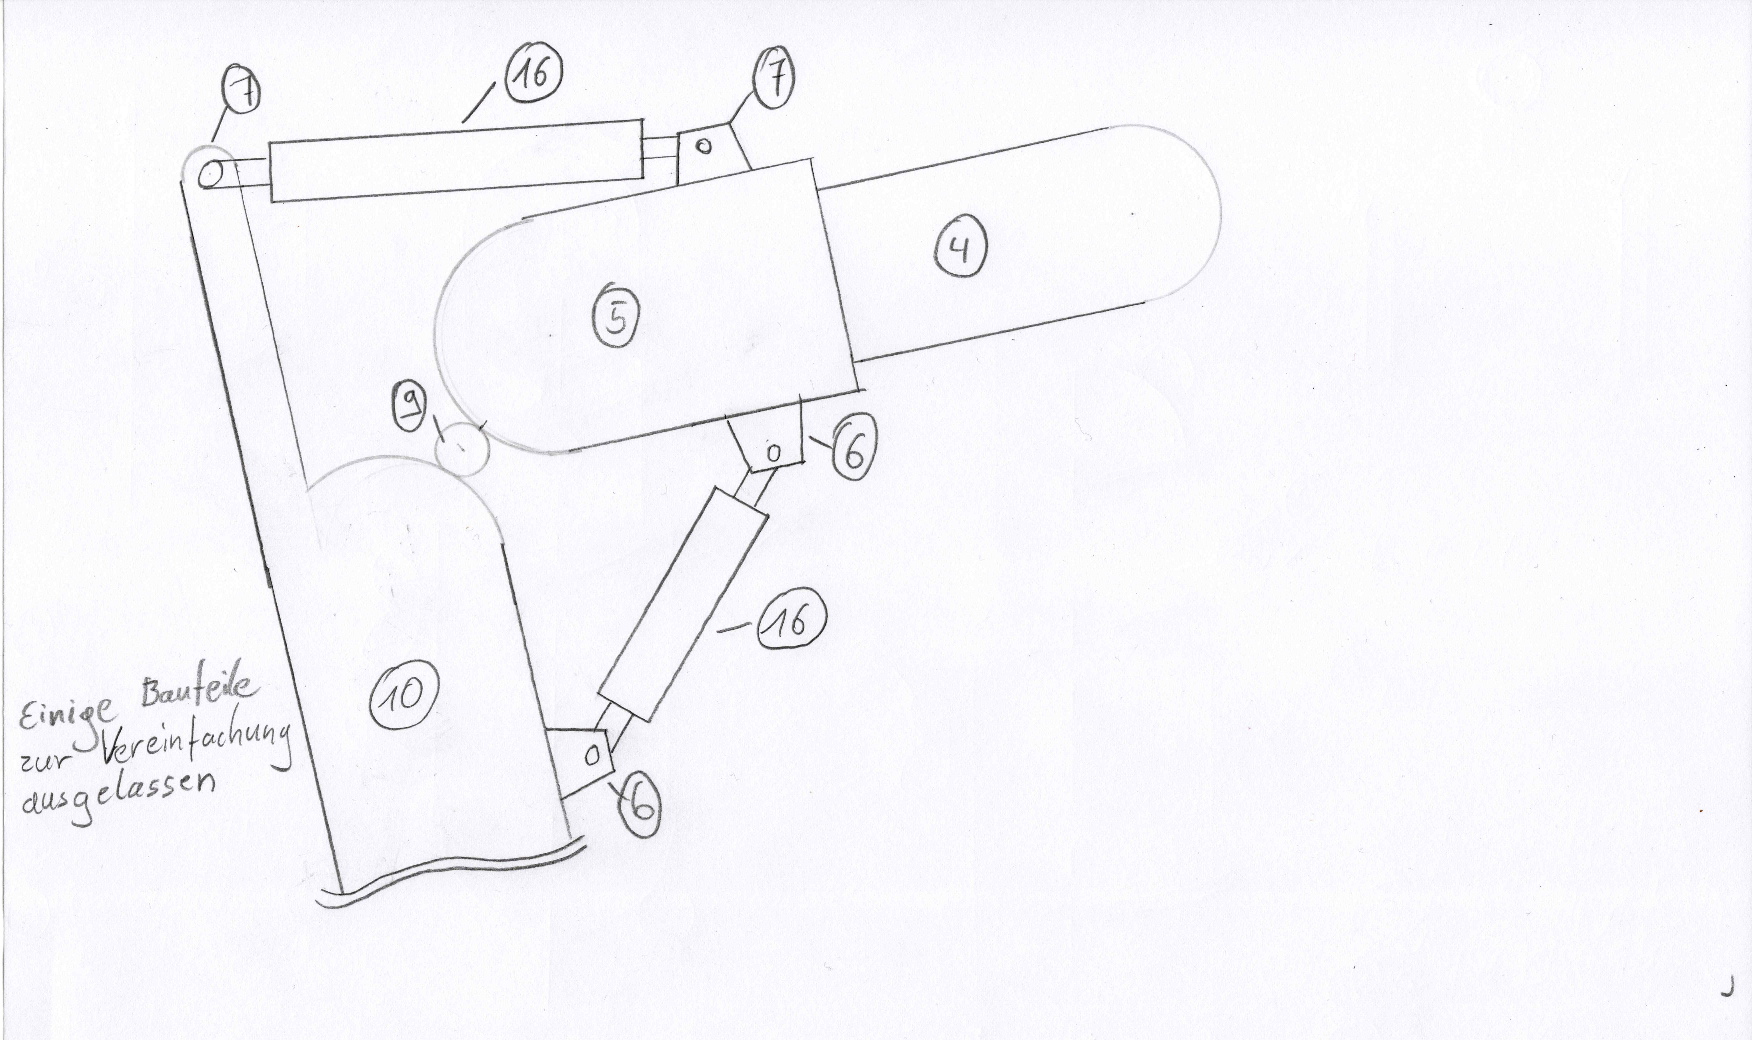
\includegraphics[width=\textwidth]{Abb/Prinzipskizze_Ellbogen}
		\caption[Prinzipskizze - Ellbogen]{Prinzipskizze -- Ellbogen.}
		\label{fig:prinzipskizze-ellbogen}
	\end{figure}

	\begin{figure}[h]
		\centering
		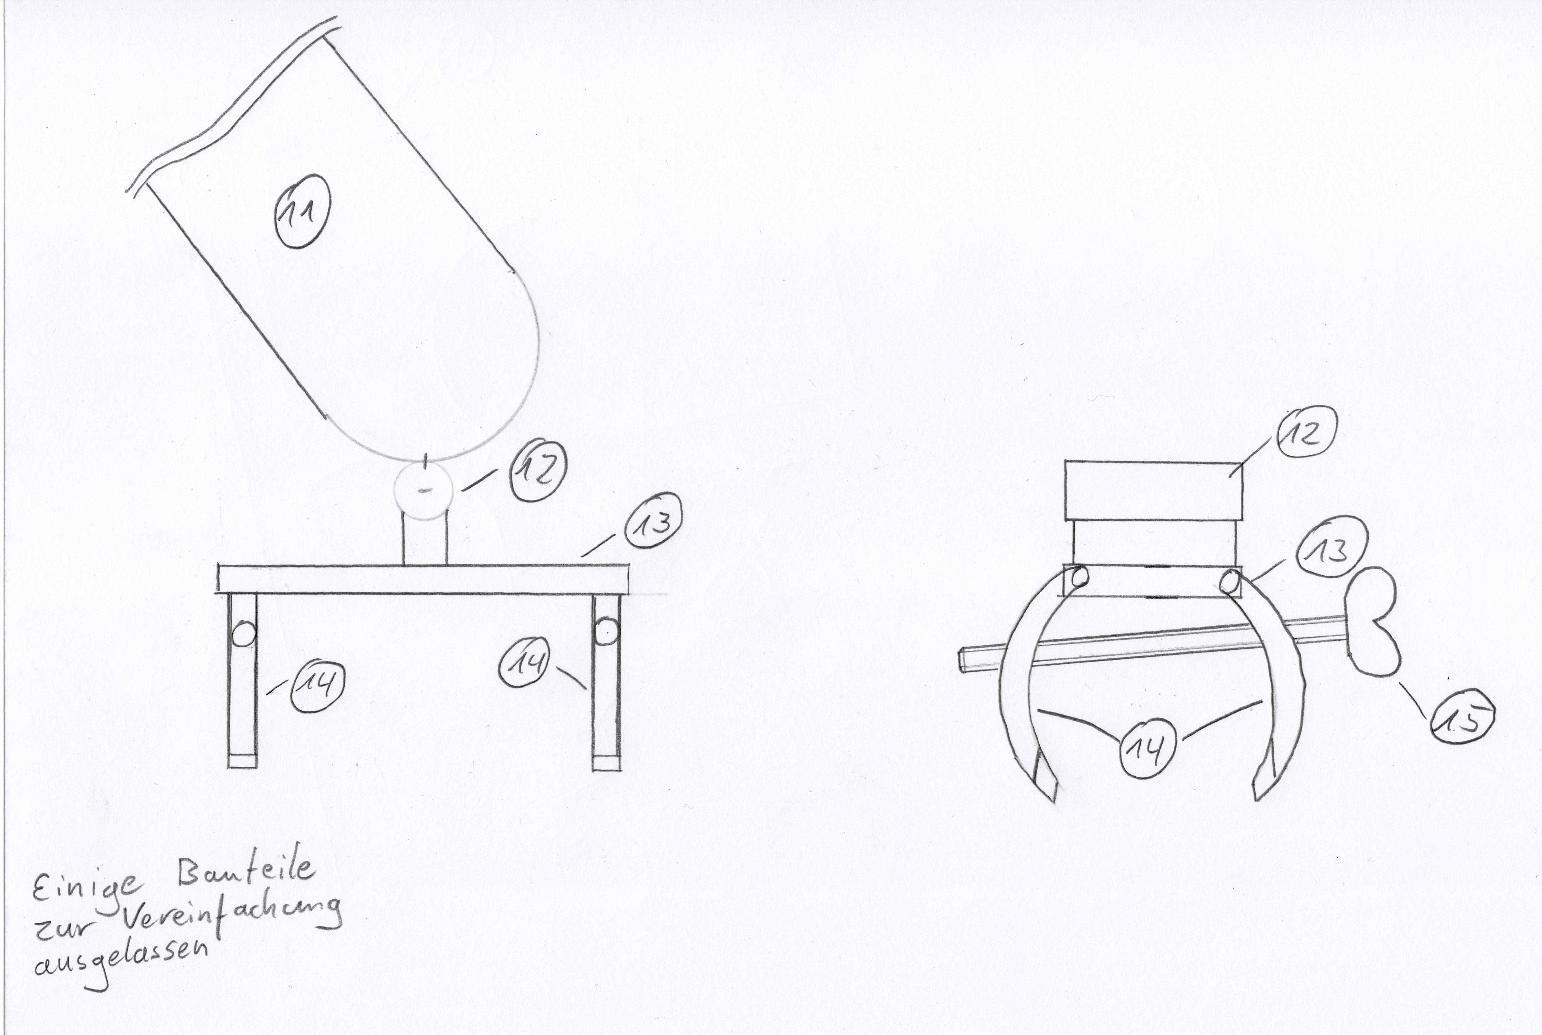
\includegraphics[width=\textwidth]{Abb/Prinzipskizze_Handgelenk_und_Hand}
		\caption[Prinzipskizze - Handgelenk und Hand]{Prinzipskizze -- Handgelenk und Hand.}
		\label{fig:prinzipskizze-handgelenk-und-hand}
	\end{figure}